\documentclass[margin=3mm]{standalone}
\usepackage{tikz}
\usetikzlibrary{shapes, arrows}

\tikzstyle{startstop} = [rectangle, rounded corners, minimum width=2cm, minimum height=1cm, text centered, draw=black, text=white, fill=black!80]
\tikzstyle{statement} = [rectangle, minimum width=4cm, minimum height=1cm, text centered, draw=black, fill=blue!20]
\tikzstyle{decision} = [rectangle, minimum height=1cm, text centered, draw=black, fill=yellow!30]
\tikzstyle{edge} = [thick, ->, >=stealth]

\begin{document}
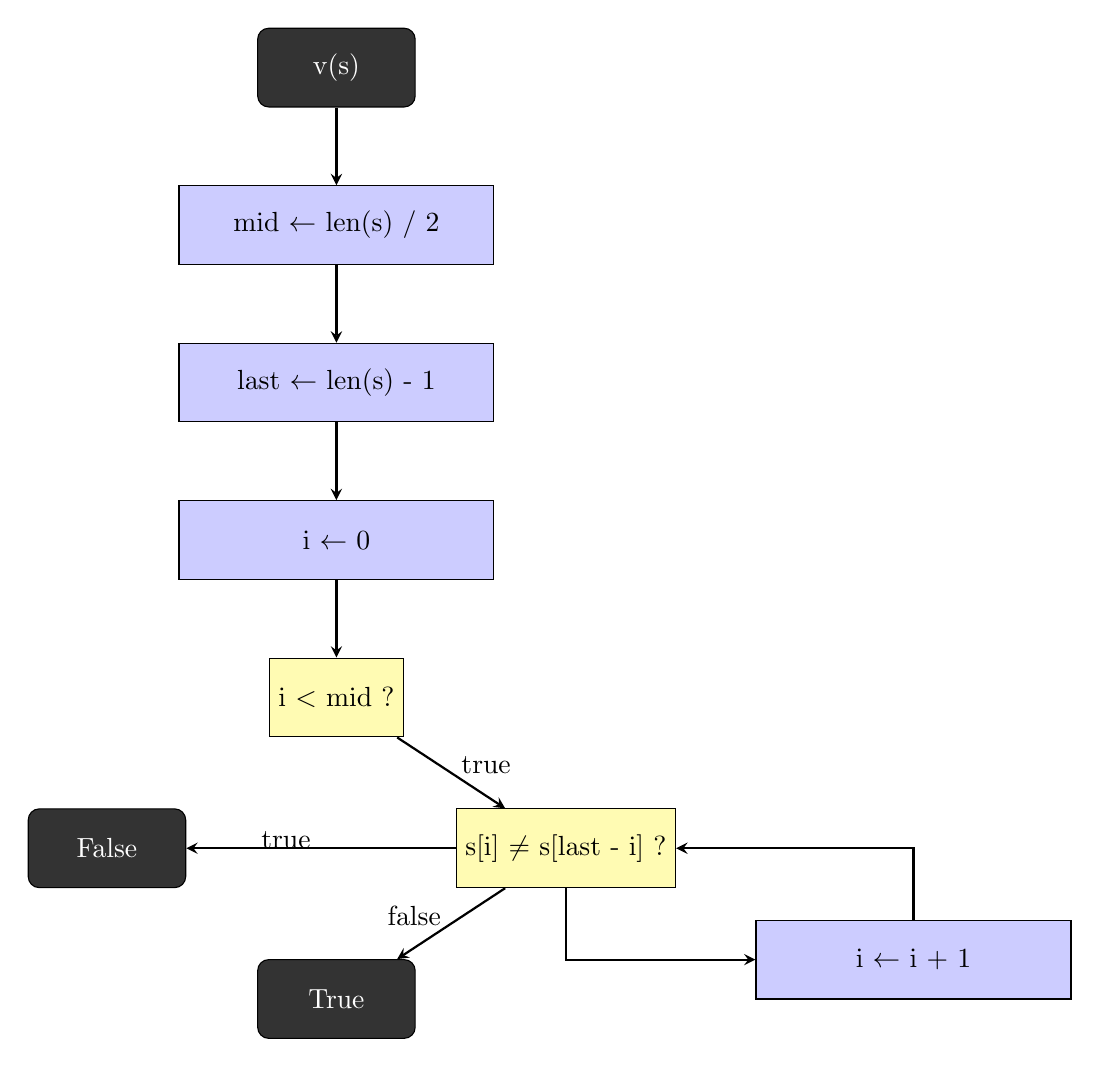
\begin{tikzpicture}[node distance=2cm]

\node (0) [startstop] {v(s)};
\node (1) [statement, below of=0] {mid $\gets$ len(s) / 2};
\node (2) [statement, below of=1] {last $\gets$ len(s) - 1};
\node (3) [statement, below of=2] {i $\gets$ 0};
\node (4) [decision, below of=3] {i $<$ mid ?};
\node (5) [decision, yshift=-0.5cm, xshift=1.5cm, below right of=4] {s[i] $\neq$ s[last - i] ?};
\node (6) [startstop, yshift=-0.5cm, xshift=-1.5cm, below left of=4] {False};
\node (7) [statement, xshift=3cm, below right of=5] {i $\gets$ i + 1};
\node (8) [startstop, yshift=-0.5cm, xshift=-1.5cm, below left of=5] {True};

\draw [edge] (0) -- (1);
\draw [edge] (1) -- (2);
\draw [edge] (2) -- (3);
\draw [edge] (3) -- (4);
\draw [edge] (4) -- node[anchor=west, yshift=0.1cm]{true} (5);
\draw [edge] (5) -- node[anchor=east, yshift=0.1cm]{false} (8);
\draw [edge] (5) |- (7);
\draw [edge] (5) -- node[anchor=east, yshift=0.1cm]{true} (6);
\draw [edge] (7) |- (5);

\end{tikzpicture}
\end{document}